\documentclass[11pt]{article}
\usepackage{amsmath}
\usepackage{graphicx}
\usepackage{subfig}
\usepackage{caption}
\usepackage{float}
\author{Francesco Saverio Zuppichini}
\title{Machine Learning - Assignment 1}
\begin{document}
\maketitle

\section{The Perceptron}
\subsection{Question 1}
\subsubsection{Vectorized equations}
The vectorized equation for a single perceptron

\begin{equation}
output = XW + b
\end{equation}
Where $X = {x_1, ... x_n}$, $W = {w_1, ..., w_n}$. We denote $y$ the output of the perceptron

\subsubsection{Mean Squared Error}
The mean squared error function for our single perceptron
\begin{equation}
	E(w) = \frac{1}{N}\sum_{i = 1}^N(\underbrace{y(x_i,w_i)}_{\text{predicted}} - \underbrace{t_i}_{\text{actual}})^2)
\end{equation}
One trick that is usual done is to multiply equation $(2)$ by $\frac{1}{2}$, so when we take the derivative the $2$ goes away. This is called One Half Mean Squared Error.

\subsubsection{Derivate of the error with respect to the weights}
In order to reduce our error function and adjust each weight we need to compute the first derivati with respect to the weights. We will use the modified version of equation $(2)$ called One Half Mean Squared Error.
\begin{equation}
\frac{\delta E}{\delta w_i}	= y - t
\end{equation}
\subsubsection{Gradient Descend}
The gradient descend is an iterative optimisation algorithm that follow the direction of the negative descent in order to find the minimum of an objective function. It is can be used as Learning Algorithm since it allows to reduce our error function, equation $(2)$, and adjust the weights properly.
It's equation
\begin{equation}
	w_{k + 1} = w_k - \eta \nabla E(w_k)
\end{equation}
Where $\eta$ is the step size, also called \textbf{learning rate} in Machine Learning. This parameter influence the behavior of Grandient Descent, a small number can lead to local minimum, while a bigger learning rate could "over-shoot" and decreaasing the converge ration. 

For this reasons, numerous improvements have been proposed to avoid local minima and increase its convergence ration. Some of them are: Conjugate Gradient and Momentum.
% TODO if time talk about them
\subsection{Implement the MSE and dMSE}
You can find them in \emph{MSE.py}
\subsection{Implement the function forward and backward}
For the \emph{forward} and \emph{backward} function you can find the code in \emph{Perceptron.py}. You can find \emph{train\_one\_step}in \emph{sketron.py}.

\subsection{Implement the \emph{run\_part1}}
You can find the implementation in the code. The plot showed in figure \ref{fig:runPart1} the final result after 15 steps using a learning rate of $0.02$
\begin{figure}[H]
	\centering
	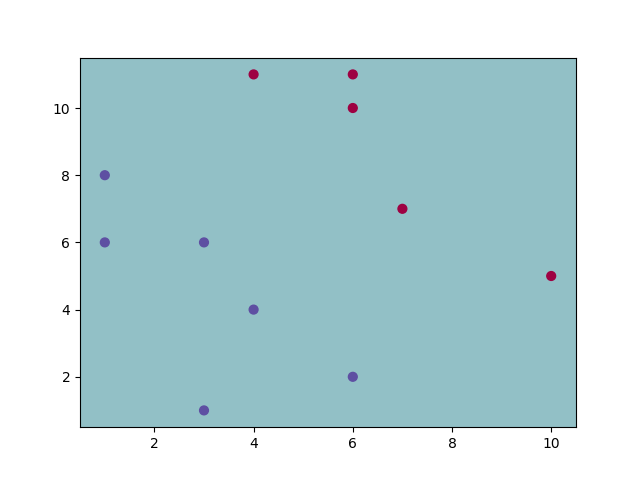
\includegraphics[scale=0.5]{images/run_part1}
	\caption{\emph{run\_part1} plot}
	\label{fig:runPart1}
\end{figure}

\section{A Neural Network}
\subsection{ Implement the activation functions}
You can find them inside \emph{activation.py}
\subsection{Question 2}
\subsubsection{Forward pass}
In order to calculate the forward pass of a Neural Network we need to compute the activation of each layer, $l$, ad use it as input of the next one until we reach the output layer.

Equation \ref{eq:forwardPass} shows the activation $a$ of layer $l$ for the $j$-th neuron on that layer.

\begin{equation}
\label{eq:forwardPass}
a^l_j = \sigma(\sum_k w^l_{jk}a^{l-1}_k + b^l_j)
\end{equation}

Where $w^l_{jk}$ is the connection from neuron $k$ in the $l-1$ layer to $j$, $a^{l-1}$ is the activation of the previous layer and $b^l_k$ is the bias of $k$-th neuron in the $l$ layer. With this in mind, we can rewrite \ref{eq:forwardPass} in a efficient vectorized form
\begin{equation}
\label{eq:forwardPassVectorized}
a^l = \sigma(W^la^{l-1} + b^l)
\end{equation}

\subsubsection{delta rules}
A Neural Network try to change its weights in order to decrease the error function, $E$. We define $\delta^l_j$ the output error of neuron $j$ in layer $l$
\begin{equation}
	\label{eq:deltaRule_1}
	\delta^l_j = \frac{\delta E}{\delta z^l_j}
\end{equation}
Stringly speaking, $\delta^l_j$, is how much the error function changes by changing the weighted input on that layer. Applying the chain rule, equation \ref{eq:deltaRule_1} becomes
\begin{equation}
\label{eq:deltaRule_2}
\delta^l_j = \frac{\delta E}{\delta a^l_j} \frac{\delta a^l_j}{\delta z^l_j}
\end{equation}
Knowning that $a^l_j = \sigma(z^l_j)$ equation \ref{eq:deltaRule_2} can be rewritted
\begin{equation}
\label{eq:deltaRule}	
\delta^l_j = \frac{\delta E}{\delta a^l_j} \sigma'(z^l_j)
\end{equation}  

 %
%We define $\Delta z^l_j$ the quantity added to the $j$-th neuron's weighted input in the $l$ layer by the network.
% The new output of that neuron becomes $\sigma(z^l_k + \Delta z^l_j)$ causing a changing by $\frac{\delta E}{\delta z^l_k}\Delta z^l_j$. 
\subsubsection{Derivatives of the weights}
We want to compute $\frac{\delta E}{\delta w^l_{jk}}$. Applying the delta rule
\begin{equation}
\frac{\delta E}{\delta w^l_{jk}} = \frac{\delta E}{\delta z^l_j}\frac{\delta z^l_j}{\delta w^l_{jk}} =	
\frac{\delta E}{\delta a^l_j}\frac{\delta a^l_j}{\delta z^l_{j}}
\frac{\delta z^l_j}{\delta w^l_{jk}}
\end{equation}
\begin{equation}
\label{eq:derivativesWeigthDeltas}	
\frac{\delta E}{\delta w^l_{jk}} = a^{l-1}_k \delta^l_j
\end{equation}
\subsection{Implement the functions forward and backward of the Neural Network class.}
\subsection{Train Network}
I decide to split my Training set and Test set by a ratio of 80:20. Figure METTI FIGURA shows the converge of the network with different steps size on the training set, while Figure DIOCANE FIGURE shows it on the test set.

\end{document}
